%-------------------------------------------------------------------------------
\documentclass[openany]{ufsctex/ufsctex}
%-------------------------------------------------------------------------------
% Packages

% Translation\usepackage{pdfpages} 

\usepackage[brazil]{babel}
\usepackage[utf8]{inputenc}
\usepackage{hyperref}
\usepackage{pdfpages}
\usepackage{listings}
\usepackage{longtable}
\usepackage{graphicx} % Possibilita o uso de figuras e gráficos

% General
\usepackage{color}  

 
\definecolor{codegreen}{rgb}{0,0.6,0}
\definecolor{codegray}{rgb}{0.5,0.5,0.5}
\definecolor{codepurple}{rgb}{0.58,0,0.82}
%-------------------------------------------------------------------------------
% User-commands
\newcommand{\todo}[1]{{\color{red}{#1}}}

%-------------------------------------------------------------------------------

\instituicao[a]{Universidade Federal de Santa Catarina} % Opcional
\departamento[a]{Departamento de Informática e Estatística}
\curso[o]{Ciências da Computação}
\documento[o]{Trabalho de conclusão de curso} % [o] para dissertação [a] para tese
\subtitulo{Trabalho Individual 3}
\titulo{Segurança em Computação}
%\subtitulo{Subtítulo (se houver)} % Opcional
\autor{Leonardo Schlüter Leite}
\grau{Bacharel em Ciências da Computação}
\local{Florianópolis} % Opcional (Florianópolis é o padrão)
\data{30}{abril}{2019}


\begin{document}
    \folhaderosto
    \sumario
    
\chapter{Respostas}
    \section{Questão 1}
    Foram utilizados os seguintes comandos em bash, no terminal do Ubuntu 18.04. Estes comandos foram retirados do site fornecido https://help.ubuntu.com /community/GnuPrivacyGuardHowto
    
\begin{lstlisting}[language=bash,breaklines=true, tabsize=2,basicstyle =\fontsize{9}{11}]
  1. gpg --gen-key //aqui foram inseridos as infos necessarias para criar o certificado e a chave
  2. export GPGKEY=62E6B6A3
  3. gpg -armor --export leonardoschluter@gmail.com > mykey.asc // utilizado para exportar minha chave publica
\end{lstlisting}


O Resultado destes comandos foi um certificado(leonardoschluter@gmail.com), uma chave privada, uma chave pública(KeyID: 62E6B6A3) e o arquivo mykey.asc. O conteúdo deste arquivo foi depois utilizado para publicar o certificado no Servidor de chaves PGP do CAIS.

	\section{Questão 2}
		Até a etapa de publicar o certificado criado o processo é o mesmo da questão anterior. Sendo que agora o KeyID é 9229C802, o email utilizado permanece o mesmo. Agora, para criar o certificado de revogação, importá-lo e depois publicar no servidor de chaves PGP do CAIS foram utilizados os seguintes comandos em bash, no terminal do Ubuntu 18.04:
		
\begin{lstlisting}[language=bash,breaklines=true, tabsize=2,basicstyle =\fontsize{9}{11}]
  1. gpg -o certificado_revogado.asc --gen-revoke -armor 9229C802
  2. gpg --import certificado_revogado.asc 
  3. gpg --keyserver keyserver.cais.rnp.br --send-keys 9229C802
\end{lstlisting}

	
A Figura \ref{fig:a} mostra o resultado da questão 1 e 2.


\begin{figure}[!htb]
   \centering
   \caption{KeyIDs geradas no servidor de chaves PGP do CAIS.}\label{fig:a}
   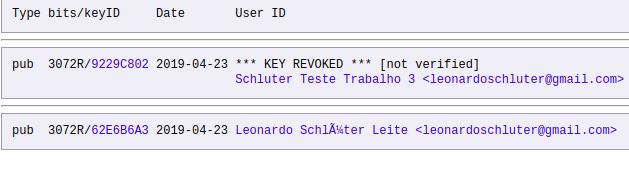
\includegraphics[scale=0.6]{images/questao2.png}
\end{figure}

\section{Questão 3}

	Primeiro é necessário assinar algum certificado. Para este exemplo usaremos o KeyID 1C0AAEB4 do colega Joaquim Boschini. Para realizar a assinatura do certificado, primeiro precisamos baixar a chave, importá-la, depois realizar a assinatura e enviar novamente para o servidor de chaves(o ideal é mandar a assinatura para o dono da chave, para que o mesmo possa publicá-la).Para isso foi utilizado os seguintes comandos em bash:
	
\begin{lstlisting}[language=bash,breaklines=true, tabsize=2,basicstyle =\fontsize{9}{11}]
  1. gpg --recv-keys 0x1C0AAEB4
  2. gpg --fingerprint 1C0AAEB4 // utilizado para verificar se realmente eh o certificado que eu queria
  3. gpg --sign-key 1C0AAEB4
  4. gpg -o joaquimSigned.asc --armor --export 1C0AAEB4
  5. gpg --keyserver keyserver.cais.rnp.br --send-keys 1C0AAEB4
\end{lstlisting}

	Depois para revogar a assinatura no certificado do colega, utilizamos o comando gpg --edit-key, que permite a execução de alguns comandos próprios. Dentro do ambiente do edit-key utilizamos o comando >revsig para justamente revogar a assinatura e o comando >save para, obviamente, salvar. Depois disso publicamos a revocação utilisando o comando --send-keys. Podemos observar na figura \ref{fig:a3} que o certificado foi assinado pela minha chave (KeyID 62E6B6A3) e depois a assinatura foi revogada.
	
	
\begin{figure}[!htb]
   \
   \caption{Assinaturas do KeyID 1C0AAEB4}\label{fig:a3}
   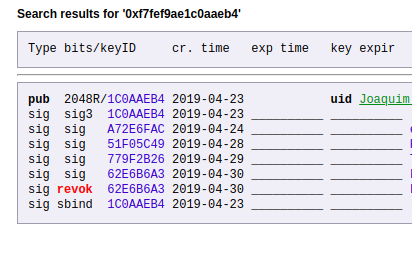
\includegraphics[scale=0.6]{images/questao3.png}
\end{figure}

\section{Questão 4}
	Um anel de chaves privadas é, segundo a wiki do GNOME, uma coleção de componentes que guarda senhas, chaves, certificados e disponibiliza o que está guardado com outras aplicações. o Anel de chaves do GNOME é implementado para seguir o padrão PKCS\#11, que define como chaves e certificados devem ser manejados. O Keyring no ubuntu fica localizado em .local/share/keyrings. Teoricamente apenas o usuário que criou o keyring tem acesso. Este acesso se dá através de sessão.
	
\section{Questão 5}
	Assinar localmente faz com que apenas o meu keyring contenha esta assinatura para a chave x. Enquanto assinar no servidor replica para todos os outros servidores GPG, assim replicando a assinatura para todas as replicas online.

\section{Questão 6}
	
	
\section{Questão 7}
	Subchaves são como as chaves normais, porém está ligada à um par de chave mestre, segundo a wiki do Debian.Porntato, pode-se usá-las como as chaves normais. Servem principalmente para evitar que você utilize seu par de chaves mestre para coisas do dia a dia. Assim evitando que: se algo aconteça à chave que você usa no dia a dia, você não perca sua identidade online, já que seu par de chaves mestre é tudo, no mundo online.
	
\section{Questão 8}
	Para adicionar uma foto à chave, utilizamos o comando gpg --edit-key, que permite a execução de alguns comandos próprios. Dentro do ambiente do edit-key utilizamos o comando >addphoto, então informar o endereço da imagem desejada. Após feito isso, basta salvar e enviar novamente a chave para o servidor de chaves.
	
\section{Questão 9}
	
\section{Questão 10} 
	Para tornar sigiloso ao público um arquivo txt, por exemplo, basta que você tenha acesso a chave pública do destinatário. Tendo essa chave pública, basta executar um comando em bash: 
		
\begin{lstlisting}[language=bash,breaklines=true, tabsize=2,basicstyle =\fontsize{9}{11}]
  1. gpg --output arquivoExemplo.txt.gpg --encrypt --recipient meu.colega.deturma@ufsc.br.com  arquivoExemplo.txt
\end{lstlisting}

	Depois, basta enviar o arquivExemplo pela internet e o outro lado vai conseguir descriptografar utlizando o seguinte comando:
			
\begin{lstlisting}[language=bash,breaklines=true, tabsize=2,basicstyle =\fontsize{9}{11}]
  1. gpg --output arquivoExemplo.txt --decrypt arquivoExemplo.txt.gpg 
\end{lstlisting}

	
\section{Questão 11}
	Para assinar um documento, é um tanto quanto fácil através do terminal. Basta usar o comando "gpg --output arquivoExemplo.sig --sign arquivoExemplo". Para assinar sem anexar ao documento, basta adicion "detach-" na frente do "sign", assim:"gpg --output arquivoExemplo.sig --detach-sig arquivoExemplo".
	
	
	Agora para verificar é mais fácil ainda, quando for uma assinatura no próprio documento, basta usar o comando: gpg --verify arquivoExemplo.sig. Se for uma assinatura separada do documento, basta informar os dois arquivos, o da assinatura e o do documento, assim: gpg --verify arquivoExemplo.sig arquivoExemplo
	

	
\end{document}
